%File: main.tex  (Social fidelity paper, AAAI 2027 format)
%
% To produce the ANONYMOUS submission version, uncomment the next line:
\def\aaaianonymous{true}
%
\documentclass[letterpaper]{article} % DO NOT CHANGE THIS

\ifdefined\aaaianonymous
    \usepackage[submission]{aaai2027}
\else
    \usepackage{aaai2027}
\fi

\usepackage{times}  % DO NOT CHANGE THIS
\usepackage{helvet}  % DO NOT CHANGE THIS
\usepackage{courier}  % DO NOT CHANGE THIS
\usepackage[hyphens]{url}  % DO NOT CHANGE THIS
\usepackage{graphicx} % DO NOT CHANGE THIS
\urlstyle{rm} % DO NOT CHANGE THIS
\def\UrlFont{\rm}  % DO NOT CHANGE THIS
\usepackage{natbib}  % DO NOT CHANGE THIS AND DO NOT ADD ANY OPTIONS TO IT
\usepackage{caption} % DO NOT CHANGE THIS AND DO NOT ADD ANY OPTIONS TO IT
\usepackage{booktabs} % for tables
\frenchspacing  % DO NOT CHANGE THIS
\setlength{\pdfpagewidth}{8.5in} % DO NOT CHANGE THIS
\setlength{\pdfpageheight}{11in} % DO NOT CHANGE THIS

\pdfinfo{
/TemplateVersion (2027.1)
}

\setcounter{secnumdepth}{0} % AAAI: no section numbers

% ---- Title (Title Case, per AAAI) ----
\title{When Truth Loses Its Source: Provenance-Aware Memory for Socially Distributed Agents}

\author{
    Gwyneth Sanford \\ % PLACEHOLDER author list --- TBD
}
\affiliations{
    Affiliation TBD \\
    author@example.com
}

\begin{document}
\maketitle

\begin{abstract}
LLM agents increasingly coordinate by talking to one another, and a growing body of work
shows that information \emph{spreads} through agent societies. We ask a reliability question
that spread does not answer: when a ground-truthed fact changes, does the society come to
\emph{hold} the new truth, or merely \emph{say} it? With a social-fidelity probe that
separately measures what agents hear, say, and later hold, we find a robust speech--belief
dissociation: an authoritative source drives agents to utter the current value while their
held belief stays at baseline. No natural lever fixes this---not model capability,
connectivity, memory swaps, richer personas, or a persistent source; only direct broadcast, an
overwrite control, succeeds. The mechanism is path-dependent entrenchment: the version
established early and broadly wins. We then localize the repair to a single architectural
choice---integrating heard claims by \emph{provenance} (source and version) rather than by
frequency. Provenance-aware memory (PROV) is the only memory architecture that lifts held
truth, and it holds across scenarios, fact types, topologies, and model families
($n{=}8$). Hardened into an auditable architecture (APM) with origin anchoring, corroboration,
and abstain, it remains the only architecture that survives an adversarial liar (zero hijack,
against PROV's collapse) and settles to a realistic, non-saturating equilibrium under sparse
communication---never confidently wrong.
\end{abstract}

% ============================================================
\section{Introduction}
A true update can become unreliable without ever becoming intentionally false. In human
societies a message may be accurate when first announced, but after a few retellings people
keep the content while losing track of who said it, when it was updated, and whether it
superseded an older version. This is the telephone-game failure: the social channel does not
merely transmit content, it also drops source, timing, and authority cues.

LLM-agent societies reproduce this failure in an instrumented setting. Unlike a human rumor
chain, an agent society exposes every utterance, every injected update, every memory snapshot,
and every final answer---letting us separate three objects that are usually conflated:
\textbf{reach} (whether the current update appears in the social transcript), \textbf{speech}
(whether agents later utter the current value), and the \textbf{held answer} (whether agents
answer with the current value when probed after transmission).

Generative-agent work establishes that information can spread through an agent society
\citep{park2023generative,li2023camel,wu2023autogen,zhou2024sotopia}. Spread, however, is not
fidelity. A correction, schedule change, or policy update can reach the conversation stream yet
fail to become the society's later answer. This is the distinction between reach and fidelity,
long drawn in misinformation research \citep{lazer2018science,vosoughi2018spread}. Our central
finding is that reach and speech improve \emph{without} durable held truth---so ``information
spread'' is not a sufficient evaluation target for agent societies.

\noindent We make three contributions:
\begin{itemize}
\item a \textbf{measurement shift}: a social-fidelity probe that separates what agents hear,
  say, and later hold after a ground-truthed update;
\item a \textbf{diagnosis}: a speech--belief dissociation driven by path-dependent
  entrenchment, which no natural lever repairs; and
\item a \textbf{cure and an architecture}: integrating by provenance rather than frequency is
  the lever that works, and hardened as APM it is the only memory architecture that stays
  interpretable, survives an adversarial liar, and yields a realistic non-saturating
  equilibrium.
\end{itemize}

Our working hypothesis is that truth decays not merely because content changes, but because
content loses its source. Stripped of source and version, ``Saturday at the porch'' and
``Sunday at the community center'' compete as undifferentiated text, and the old value can win
simply because it was established early, repeated often, or retrieved more easily. Provenance
changes the social state representation: an agent can ask not only ``what have I heard?'' but
``who said it, is it the latest authoritative version, and does it supersede the old one?''

% ============================================================
\section{Related Work}
\textbf{Agent societies and communicative agents.} Generative Agents
\citep{park2023generative}, CAMEL \citep{li2023camel}, AutoGen \citep{wu2023autogen}, and
SOTOPIA \citep{zhou2024sotopia} establish the setting: agents talk, remember, coordinate, and
simulate social environments. We pose a missing reliability question within it---the fidelity
of a \emph{changing} held fact.

\textbf{Misinformation, rumor, reach vs fidelity.} Rumor and continued-influence research
separates spread from truth and shows that corrections often fail to displace stale beliefs
\citep{lewandowsky2012misinformation,thorson2016belief}. LLM-agent rumor simulations are close
neighbors, but they typically measure propagation or vulnerability; we measure held-fact
fidelity after a truth change. The closest concurrent neighbor \citep{xie2026spark} also
studies provenance-style cures and adoption-vs-repetition; we lead instead on the explicit,
separately elicited say/hold dissociation, a head-to-head decentralized-memory comparison, and
adversarial robustness.

\textbf{Factuality and measurement.} Treating truthfulness as a semantic behavioral target
rather than surface fluency is now standard \citep{lin2022truthfulqa,manakul2023selfcheckgpt,
farquhar2024detecting}. Our three-way verdict mirrors fact verification
\citep{thorne2018fever} and the efficacy-vs-locality structure of knowledge editing
\citep{meng2022rome,meng2023memit}.

\textbf{Memory, correction, recursive degradation.} Memory systems
\citep{chhikara2025mem0,xu2025amem,zhong2024memorybank} explain why exposure is not retention;
belief revision and truth maintenance \citep{alchourron1985logic,doyle1979truth} and
source-credibility opinion dynamics \citep{degroot1974reaching} motivate provenance; and
model-collapse work \citep{shumailov2023curse} offers an analogy for recursive
degradation---though ours is communication-time degradation, not training-time collapse.

% ============================================================
\section{Method: The Social-Fidelity Probe}
\textbf{Setup.} A society of $N{=}25$ LLM agents on a contact graph organizes an event. At
round~1 the event's time and place \emph{change} from a stale value (A) to a current value (B),
and the update is injected into a single source agent. Agents then meet pairwise over rounds (a
\texttt{meetings} parameter sets how many encounters each agent has per round, i.e.\
connectivity), converse, store what they hear, and retrieve memory to condition later
utterances. We log every utterance (SAID) and, at the end, privately interview every agent
about the current fact (HELD): Inject $\rightarrow$ Propagate $\rightarrow$ Measure.

\textbf{The current / stale / unknown verdict.} Because the fact's truth value changed, we
classify each held answer three ways, mirroring recognized evaluation structures:
\textbf{current} (holds the new value---edit \emph{efficacy} / \textsc{supported}),
\textbf{stale} (holds the superseded value---a \emph{locality} failure / continued-influence),
and \textbf{unknown} (holds neither---a retention failure / \textsc{not-enough-info}). The
three-way split is load-bearing: separating \emph{stale} (active corruption) from \emph{unknown}
(information loss) is essential, because interventions act on them differently---scaling
capability, for instance, converts loss into confident corruption. A semantic LLM judge
reproduces the keyword verdict (99--100\% agreement), so the categories are not a keyword
artifact.

\textbf{HEARD / SAID / HELD.} The probe's leverage comes from separating what reaches an agent,
what it utters, and what it later holds. ``Held belief'' is operational---the answer an agent
gives when probed; we make no claim about literal mental states.

% ============================================================
\section{Results}

\subsection{Social Fidelity Decays, and No Natural Lever Repairs It}
In the core task the current value reaches the conversation stream but does not reliably become
the society's held answer. Over a long horizon the dynamics are sharper still: current truth can
rise early, peak near round~6, then decay toward a low steady state by round~30---so truth can
appear transiently and still lose, and the round-5 snapshot slightly overstates retention.

Figure~\ref{fig:levers} and Table~\ref{tab:levers} rule out every intuitive repair. Capability
(16$\to$21\% across mini$\to$gpt-5.4$\to$gpt-5.5), connectivity (roughly neutral in the powered
rerun---the early ``connectivity amplifies corruption'' cell was an underpowered outlier, now
retracted), a memory swap (the apparent rescue did not replicate), thick personas, and a
persistent authoritative source all leave held truth at the $\sim$14--21\% baseline. Only
broadcasting the current value into \textbf{every} agent succeeds (99\%)---an overwrite-style
positive control that bypasses social transmission, not a social cure. Agents can clearly output
the truth; the problem is that ordinary social communication does not reliably install it as
held belief.

\begin{figure}[t]
\centering
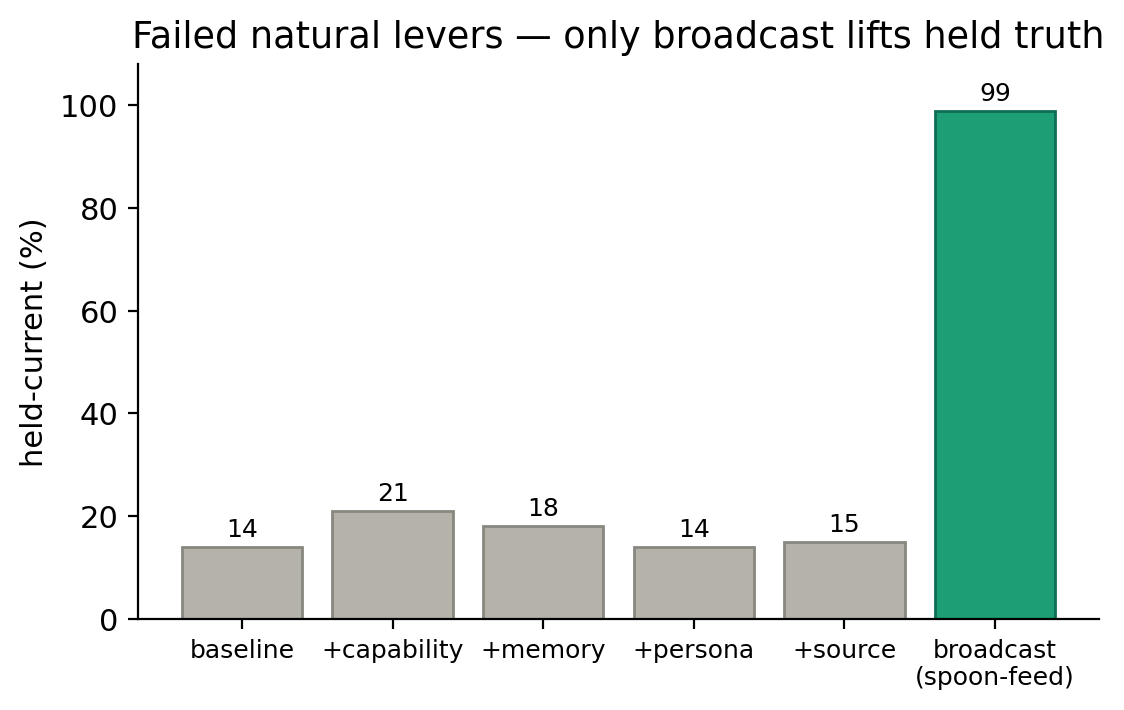
\includegraphics[width=\columnwidth]{figures/fig_failed_levers.png}
\caption{Failed natural levers. Capability, memory, persona, and an authoritative source all
leave held truth at baseline; only broadcast (an overwrite control) succeeds.}
\label{fig:levers}
\end{figure}

\begin{table}[t]
\centering
\caption{Failed-lever evidence ledger (held-current; ns = not significant).}
\label{tab:levers}
\begin{tabular}{lcc}
\toprule
Lever & Contrast & Held-current \\
\midrule
Capability   & mini$\to$gpt-5.5      & 16$\to$21\% (ns) \\
Connectivity & meetings 1/2/3        & ratio $\sim$1.0 (ns) \\
Memory       & GA vs.\ smga3g        & $\Delta\approx0$ (ns) \\
Persona      & thin vs.\ thick       & 12 vs.\ 14\% (ns) \\
Source       & vs.\ baseline         & $\Delta{+}0.8$ (ns) \\
Broadcast    & vs.\ baseline         & $\Delta{+}21.8 \to 99\%$ \\
\bottomrule
\end{tabular}
\end{table}

\subsection{Speech Is Not Belief}
Figure~\ref{fig:dissoc} is the centerpiece. Separating SAID (final-round utterances) from HELD
(private interviews) exposes a dissociation: under a persistent authoritative source, agents
reach 83\% current in what they \textbf{say} while their \textbf{held} belief stays near
baseline (15\%). The gap is not confined to the source condition---even baseline agents say the
current value more than they hold it (SAID 56\% / HELD 12\%)---and only broadcast aligns the two
(99/99). Reach is not belief: a fact can be visible in the transcript while failing as held
state. The pattern replicates across three scenarios and survives thick personas.

\begin{figure}[t]
\centering

\includegraphics[width=\columnwidth]{figures/fig_say_vs_hold.png}
\caption{Speech is not belief. A source pushes SAID to 83\% while HELD stays at 15\%; even
baseline says more than it holds; only broadcast aligns the two.}
\label{fig:dissoc}
\end{figure}

\subsection{The Mechanism Is Entrenchment, Not Recency}
Two stories could explain a sticky stale belief. If \emph{recency} drove belief, a late
all-agent broadcast just before the probe should work; if \emph{repetition} drove it, a single
early all-agent broadcast should fail. The opposite happens (Figure~\ref{fig:mech}): an early
(round-1) all-agent correction succeeds (100\%), while an identical late (round-5) one fails
(0\%). What governs the outcome is whether the truth becomes the early, broad version that later
conversation reinforces. The stale value starts with incumbent advantage, so a narrow or late
correction can be uttered without ever taking over the society's held state. We call this
path-dependent entrenchment.

\begin{figure}[t]
\centering

\includegraphics[width=0.85\columnwidth]{figures/fig_entrenchment.png}
\caption{Entrenchment, not recency. An early all-agent correction succeeds (100\%) while an
identical late one fails (0\%).}
\label{fig:mech}
\end{figure}

\subsection{The Cure: Integrate by Provenance, Not Frequency}
The diagnosis points to a precise repair. Decay arises because integration is by frequency, so
the stale incumbent wins; we integrate by \emph{provenance} instead. Each claim carries a
version (its origin round) as conversation metadata; an agent holds the highest version it has
\emph{heard} and re-broadcasts that versioned belief, so the latest authoritative version
supersedes the merely frequent older one. This is \emph{fair}, not broadcast in disguise: PROV
never overwrites an agent---the current value must still arrive through conversation, and an
agent that never hears it stays stale or unknown. PROV changes only how an agent integrates and
relays what it locally hears. It is also principled: it directly negates the diagnosed
mechanism, it is normatively correct for a changing fact (frequency is the wrong cue---an old
value repeated often is still old), and it instantiates classic ideas---truth maintenance and
belief revision \citep{doyle1979truth,alchourron1985logic} and source-weighted opinion dynamics
\citep{degroot1974reaching}---in the social channel.

Figure~\ref{fig:arch} places PROV beside recognized memory architectures under one harness. Raw
(14), Mem0 (18), A-MEM (19), GA (22), GA-curr (25), and MemBank (25) all fail; only PROV lifts
held truth (57\%). The decisive lever is the listener-side \textbf{integration rule}, not a
larger or fancier memory.

\begin{figure}[t]
\centering

\includegraphics[width=\columnwidth]{figures/fig_architecture.png}
\caption{Architecture comparison ($n{=}8$). Recognized memories all fail (14--25\%); only PROV
lifts held truth (57\%).}
\label{fig:arch}
\end{figure}

The cure is not a single-condition artifact (Table~\ref{tab:general}): PROV wins across three
scenarios, a numeric fact change (dues \$40$\to$\$60), and contact topologies, with the margin
\emph{widening} on harder structured networks.

\begin{table}[t]
\centering
\caption{Generality and capability (held-current \%, GA vs.\ PROV).}
\label{tab:general}
\begin{tabular}{llcc}
\toprule
Axis & Condition & GA & PROV \\
\midrule
Model       & mini             & 21.5 & \textbf{57} \\
            & DeepSeek         & 15.5 & \textbf{64} \\
Scenario    & repair\_drive    & 22 & \textbf{57} \\
            & book\_club       & 47 & \textbf{69} \\
            & carpool          & 18 & \textbf{59} \\
Fact type   & dues \$40$\to$\$60 & 28 & \textbf{59} \\
Topology    & random           & 22 & \textbf{93} \\
            & ring             & 6  & \textbf{68} \\
            & smallworld       & 10 & \textbf{83} \\
\bottomrule
\end{tabular}
\end{table}

\subsection{The Cure Survives Capability}
Figure~\ref{fig:cap} repeats the comparison on a different model family (DeepSeek-V4-Flash) at
full power ($n{=}8$). GA is statistically flat-and-failing across models (mini 21.5\%, DeepSeek
15.5\%, overlapping CIs), while PROV wins on both (57\% / 64\%) with CIs disjoint from GA. The
cure survives capability---the mirror image of ``the phenomenon survives capability.''

\begin{figure}[t]
\centering

\includegraphics[width=\columnwidth]{figures/fig_capability_c14.png}
\caption{Capability check ($n{=}8$). GA is flat-and-failing across model families; PROV wins on
both with disjoint CIs. Error bars are 95\% CIs.}
\label{fig:cap}
\end{figure}

\subsection{From Lever to Architecture: APM}
Naive PROV identifies the right lever but is not yet a deployable architecture: it adopts the
highest version blindly---a liar can claim version~999 and hijack the society---and it carries
only a version, not an auditable chain. We harden it into \textbf{APM} (Auditable Provenance
Memory) with three guards, each closing one gap. \emph{Origin anchoring}: an \texttt{auth} flag
is minted only at the source and relayed faithfully, so unauthenticated forgeries are rejected.
\emph{Chain corroboration}: a value is committed only after $K$ independent sources support it,
counting paths rather than value-frequency---the fix for the failure mode in which systematic
garble corroborates the stale value. \emph{Abstain}: the agent holds \emph{unknown} until that
bar is met. Because every committed belief carries a complete source$\to$version$\to$path trace,
APM is auditable by construction---something black-box memories cannot offer.

Without an adversary, APM $\approx$ PROV: interpretability is nearly free ($\sim$64\% on
DeepSeek, with 60--76\% of agents holding a fully traceable belief). Its reason to exist appears
under attack (Figure~\ref{fig:adv}). A liar broadcasting a forged high-version stale claim
collapses PROV from 57\% to 33\% and hijacks 43 of 75 agents (stale 57\%); APM is unmoved
(64\%) with \textbf{zero hijack} (stale 0), its origin anchoring rejecting the forgery
society-wide. Equivalent without an adversary, APM is the only architecture left standing with
one (Table~\ref{tab:apm}).

\begin{figure}[t]
\centering

\includegraphics[width=\columnwidth]{figures/fig_apm_adversarial.png}
\caption{Adversarial liar. PROV collapses (held 33\%, stale 57\%) while APM is unmoved (held
64\%, stale 0).}
\label{fig:adv}
\end{figure}

\begin{table}[t]
\centering
\caption{Architecture comparison including APM. Held-current is mini/$n{=}8$ for recognized
memories; APM no-adversary is on DeepSeek; the under-liar column is mini.}
\label{tab:apm}
\begin{tabular}{lccc}
\toprule
Memory & Held & Auditable & Under liar \\
\midrule
Raw     & 14 & no   & --- \\
Mem0    & 18 & no   & --- \\
A-MEM   & 19 & no   & --- \\
GA      & 22 & no   & hijacked \\
MemBank & 25 & no   & --- \\
PROV    & 57 & half & 33 (stale 57\%) \\
\textbf{APM} & \textbf{$\approx$64} & \textbf{yes} & \textbf{64 (stale 0)} \\
\bottomrule
\end{tabular}
\end{table}

\subsection{APM Does Not Saturate}
One might worry that any sticky provenance memory simply floods to 100\%. That ceiling is a
communication-model artifact (every-utterance, lossless broadcast), not a property of provenance
integration. Figure~\ref{fig:curve} sweeps communication density---how often agents actually
mention the fact. APM traces a smooth, fully monotonic S-curve: held-current climbs from 11\%
(mention~0, where only the source knows) to 87\% (mention 0.25--0.3), and reaches 100\% only at
the unrealistic dense limit (0.5+). The 40\% value at the sparse end is an honest floor, not a
ceiling. Crucially, stale stays 0 at every density: under hard sparse communication no method
spreads truth widely (the breadth advantage over GA narrows), but APM still guarantees that the
informed are never misled, which GA does not. Its safety is independent of how far truth
spreads.

\begin{figure}[t]
\centering
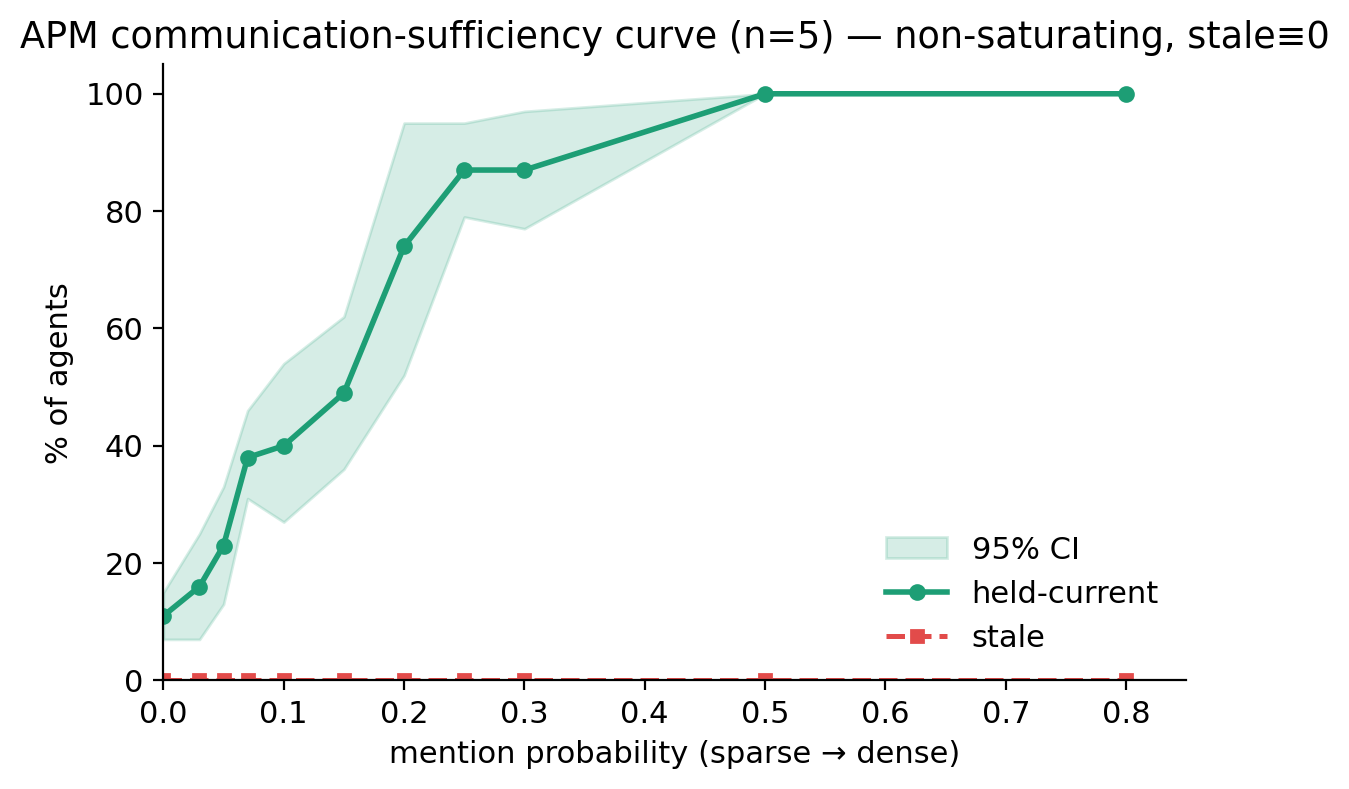
\includegraphics[width=\columnwidth]{figures/fig_apm_comms_curve.png}
\caption{APM communication-sufficiency curve ($n{=}5$). Held-current rises monotonically with
communication density and saturates only at the unrealistic dense limit; stale stays $\equiv 0$
throughout. Shaded band is the 95\% CI.}
\label{fig:curve}
\end{figure}

% ============================================================
\section{Discussion and Limitations}
\textbf{What we claim.} Social truth maintenance requires preserving provenance. PROV
demonstrates the value of provenance-aware memory; the failure of every other lever shows the
repair lives at a specific locus---listener-side integration---not in capacity. APM shows that
provenance can be hardened into an interpretable, adversary-resistant, non-saturating
architecture.

\textbf{Is structured PROV cheating?} This is the central reviewer risk, and the answer is no on
both sides. PROV is \emph{not} broadcast: it still propagates through meetings, helps only
agents the update reaches, and is weakened by loss, garble, sparse mention, horizon, and
topology. But it is \emph{not} fully naturalistic either---it assumes source and version survive
the relay as structured metadata, so it is best read as an idealized protocol or upper bound. A
companion result shows that ordinary LLM dialogue does \emph{not} spontaneously preserve
source/version, whereas an explicit attribution norm can repair held truth---a text-only upper
bound that is visibly protocolized. The engineering lesson is that agent societies may need not
larger memories but social-memory interfaces that preserve provenance through communication.

\textbf{We did not invent provenance.} Provenance is a classic idea from truth-maintenance and
belief revision. Our contribution is to (i) show that default decentralized agent memories
systematically lose it, (ii) localize the repair to the integration rule, (iii) quantify it
through the say/hold dissociation, and (iv) harden it into an auditable, adversary-tested
architecture.

\textbf{Limitations.} All experiments are simulations, and ``held belief'' is operational. APM's
headline cells are $n{=}3$--5 pilots (versus $n{=}8$ for the diagnosis and the capability check);
under sparse communication its breadth advantage over GA is suggestive (overlapping CIs) while
its safety advantage (stale 0 vs.\ 30) is decisive. APM's corroboration knob $K$ trades flooding
($K{=}1$, PROV-like) against over-conservatism ($K{\ge}2$ deadlocks without relay-before-commit),
and value fidelity remains a dependency---heavy garble still degrades it. We deliberately disable
individual forgetting so that the failure is attributable to the integration rule rather than to
memory loss; whether forgetting could itself thaw entrenchment is a question we leave to a
sequel.

\textbf{Human-society reading.} The telephone effect is not always a defect---for descriptive
social simulation, selective absorption and provenance loss are features to be reproduced, not
bugs. Our normative claim is narrower: once an agent society must maintain a changing fact for
reliable coordination, human-like telephone effects turn from feature into engineering risk.

% ============================================================
\section{Conclusion}
In a society of LLM agents, a ground-truthed update can be \emph{said} without being
\emph{held}: authority moves speech but not belief, and the version established early and broadly
entrenches. No natural lever repairs this. The repair is a specific architectural locus---
integrate heard claims by provenance, not frequency---and it holds across scenarios, fact types,
topologies, and model families. Hardened into APM, provenance integration becomes interpretable
by construction, the only architecture that survives an adversarial liar, and a realistic
non-saturating equilibrium that is never confidently wrong. Reach is not belief; for agent
societies that must track changing facts, faithfully carrying source and version is the
difference between saying the truth and holding it.

% ============================================================
\bibliography{references}

\end{document}
